\chapter{Theoretische Grundlagen}

\section{Klangsynthese}
\label{sec:orgbc9ec56}
Das wort \textbf{Synthese} bedeutet in etwa zusammensetzen oder zusammenfügen ({Duden}, 2023), beschreibt also das Erschaffen von etwas neuem durch die Vereinigung von kleineren Teilen, Klangsynthese bedeutet also, aus grundlegenden Klangwellen komplexere Klänge zu erzeugen.

Ein \textbf{Synthesizer} ist ein (meist elektronisches) Instrument, welches zur Klangsynthese fähig ist. Während die meisten herkömmlichen analogen Instrumente nur eine oder wenige unterschiedliche Klangfarben erzeugen können, ist eine der Kernaufgaben eines Synthesizers das Erzeugen von Klängen mit beliebig änderbarer Klangfarbe. Zwar können Synthesizer auch herkömmliche Instrumente imitieren, vor allem sind sie jedoch das Mittel der Wahl, wenn unnatürliche und untypische Klangfarben erzeugt werden sollen, oder wenn sich die Klangfarbe eines Tones ändern soll, während er gespielt wird.

\subsection{Klangwellen}
\label{sec:org8b72477}
Klangwellen sind die Grundbausteine der Klangsynthese. Sie können in verschiedenen Medien vorkommen, wichtig sind für uns vor allem als Spannung ausgedrückte Klangwellen, welche wir mit Elektronik manipulieren können und Schallwellen in der Luft als Endprodukt. Weitere Formen von Klangwellen sind zum Beispiel die Schwingungen einer Gitarrensaite oder Lautsprechermembran oder Elektromagnetische Wellen, zum Beispiel beim Funk.

\subsubsection{Frequenz}
\label{sec:org94a7686}
Die Tonhöhe einer Klangwelle hängt von ihrer \textbf{Frequenz} ab, also von der Geschwindigkeit, in welcher sie schwingt. Dabei nimmt das menschliche Gehirn Töne auf eine logarithmische Art und Weise wahr, um eine große Bandbreite an Tonhöhen differenzieren zu können. Deshalb entspricht ein Ton mit der doppelten Frequenz dem selben Ton eine Oktave höher. Die Einheit für Frequenzen ist \si{\hertz}, was \(\frac{1}{\si{\second}}\) entspricht, also wie oft die Welle in einer Sekunde schwingt.

\subsubsection{Amplitude}
\label{sec:org2d448b1}
Die Lautstärke einer Klangwelle korrespondiert mit ihrer \textbf{Amplitude} und wird in der Regel in Bel (bzw üblicherweise ein zehntel Bel, also Dezibel) (\si{\dB}) angegeben. Bel ist eine relative Einheit welche genutzt wird um das Energieverhältnis zweier Signale zu vergleichen.

Bei Schallwellen wird üblicherweise die Amplitude mit der kleinsten hörbaren Luftdrucksänderung (\SI{20}{\micro\pascal}) verglichen. Dadurch wird aus der relativen Einheit (dezi)Bel die Absolute Einheit \si{\dB}\textsubscript{SPL} (SPL steht für Sound Pressure Level), welche umgangssprachlich oft fälschlicherweise als \si{\dB} bezeichnet wird.

Da das menschliche Gehör Lautstärke auf eine logarithmische Art und Weise wahrnimmt, ist auch die Bel-Skala eine logarithmische. So bedeutet eine Steigerung der Lautstärke um 20 \si{\dB} eine verzehnfachung der Amplitude, also des Energieniveaus der Welle. (Siehe Abbildung unten)

\begin{figure}[htbp]
\centering
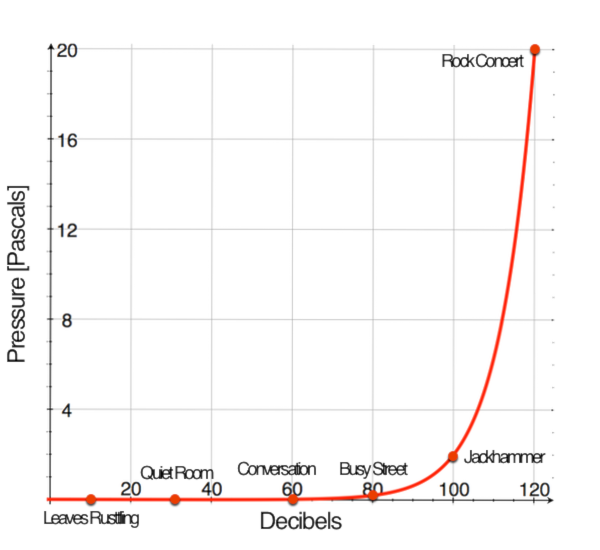
\includegraphics[height=200px]{/home/felixp/Documents/diplomarbeit/dokumentation/figures/decibel_scale.png}
\caption{Dezibelskala mit häufigen Lautstärken als Referenzpunkte (rechts) und Dezibelskala mit zugehörigen Luftdrucksänderungen in Pascal (links) ({Acoustic Today}, 2023)}
\end{figure}

Auch nimmt der Mensch gewisse Frequenzen lauter wahr als andere, Frequenzen außerhalb vom hörbaren Bereich können beispielsweise gar nicht wahrgenommen werden; deshalb kann eine Gewichtungsfunktion, genannt A-weighting, auf den Lautstärkewert angewendet werden. Dieser \textbf{Bewertete Schalldruckpegel} wird als \si{\dB}\textsubscript{A} bezeichnet und ist Standard zum Angeben gefühlter Lautstärke. (Siehe Abbildung unten)

\begin{figure}[htbp]
\centering
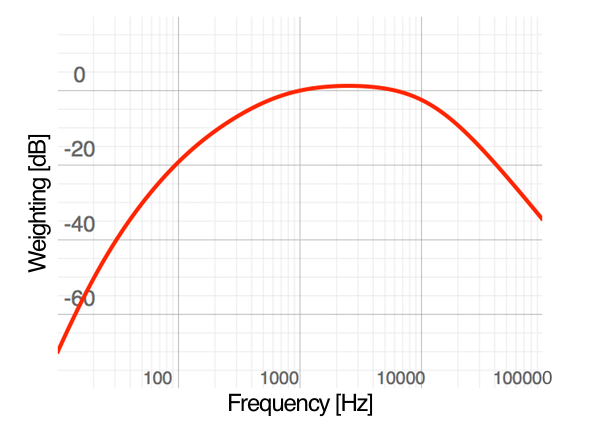
\includegraphics[width=250px]{/home/felixp/Documents/diplomarbeit/dokumentation/figures/a_weighting.png}
\caption{Gewichtungsfunktion; Hörbare Frequenzen auf der Abzisse, Hörbarkeit durch das Menschliche Gehör auf der Ordinate ({Acoustic Today}, 2023)}
\end{figure}

\subsubsection{Wellenform}
\label{sec:org4ef2151}
Klangwellen können verschiedene Formen besitzen, die grundlegende Form ist dabei eine \textbf{Sinuswelle}. Das menschliche Ohr empfindet eine sinusförmige Schallwelle als "`rein"', da sie eine einzelne Frequenz ohne \textbf{Obertöne} repräsentiert. Weitere einfache Formen sind Rechteckswellen, Sägezahnwellen und Dreieckwellen. Im Gegensatz zum Sinus besitzen diese Wellenformen viele Obertöne, welche dem Klang Farbe verleihen. Teilt die Frequenz eines solchen Obertons die Frequenz des Grundtones ganzzahlig, wird er als \textbf{Harmonisch}, also wohlklingend empfunden.

Wellenformen wie Dreieck-, Rechteck- oder Sägezahnwellen eignen sich, da sie viele Obertöne besitzen, besonders gut als Grundtöne für die subtraktive Klangsynthese.

\subsection{Klangerzeugung}
\label{sec:org19486fa}
Die für die Klangsynthese benötigten grundlegenden Klangwellen können aus verschiedensten Quellen stammen. Die häufigste davon ist wohl ein \textbf{Oszillator}, welcher durchgehende Klangwellen mit einer einfachen Wellenform wie zum Beispiel einem Sinus oder einer Rechteckswelle generiert. In einem späteren Teil dieser Dokumentation werden Aufbau und Design eines solchen Oszillators beschrieben.

Abgesehen davon können eine breite Spanne von elektronischen Musikinstrumenten / Klangquellen wie E-Gitarren, Thereminen oder Radios und Kassettenspieler die zu modifizierenden Klangwellen für einen Synthesizer bereitstellen.

\subsection{Subtraktive Klangsynthese}
\label{sec:orge25bda8}
Das Prinzip der Subtraktiven Klangsynthese besteht darin, Grundtöne mit vielen Obertönen zu filtern, um Töne mit einer gewünschten Klangfarbe zu erzeugen. Durch einen \textbf{Filter} wird die Amplitude von Teilwellen unter einer bestimmten Frequenz (=> high-pass Filter) oder über einer bestimmten Frequenz (=> low-pass Filter) verringert, wodurch zum Beispiel unangenehm hohe Obertöne gefiltert werden können.

Nach einen solchen Filter wird oft ein \ac{VCA} (siehe Abschnitt \ref{VCA}) geschalten, welcher die Amplitude des Eingangssignals proportional zur angelegten \ac{CV} (siehe Abschnitt \ref{CV}) skaliert. Diese \acl{CV} kann beispielsweise durch einen \ac{LFO} (siehe Abschnitt \ref{LFO}) oder Hüllkurvengenerator (siehe Abschnitt \ref{AR}) bereitgestellt werden. Durch einen \ac{VCA} kann einem durchgehend gleich lauten Klang Dynamik und Rhythmus verliehen werden, indem seine Lautstärke mit dem Verlauf der Zeit geändert wird.

Die meisten analogen Synthesizer basieren auf subtraktiver Klangsynthese. Üblicherweise wird dabei ein Grundton, meist aus einem Oszillator, über einen \ac{VCA} geschalten, welcher durch einen Hüllkurvengenerator angesteuert wird. Dieser Hüllkurvengenerator wird üblicherweise durch einen Sequenzer oder eine Tastatur angesteuert. Eine Abwandlung dieser grundlegenden \textbf{Signalverarbeitungskette} ist in den meisten kommerziell erhältlichen Synthesizersystemen fest verkabelt.

\subsection{Additive Klangsynthese}
\label{sec:org1cb1a73}
Nach Fourier kann jegliche Art von Wellenform durch eine Serie von Sinuswellen ausgedrückt werden. Das Prinzip der additiven Klangsynthese besteht somit darin, eine Vielzahl von Sinuswellen mit unterschiedlichen Amplituden und Frequenzen zu Kombinieren, (beispielsweise durch einen Mixer, siehe Abschnitt \ref{Mixer}) um Klänge mit jeder erdenklichen Klangfarbe zu erzeugen. Idealerweise wird jede grundlegende Sinuswelle durch eine seperate Hüllkurve moduliert um einen Klang mit laufend verändernder Klangfarbe zu erzeugen (Hannes Raffaseder, 2002). Da dies mit einer steigenden Anzahl an grundlegenden Sinuswellen eine technische Herausforderung darstellt, sind additive Synthesizer meist digital ausgeführt, ein analoges Beispiel für einen additiven Synthesizer wäre eine Orgel.

\subsection{Vocoder}
\label{sec:orgbf10125}
Ein Vocoder basiert auf dem Prinzip, ein Signal (meist eine Stimme) mittels mehrerer Band-Pass Filter in seine Frequenzbestandteile aufzuteilen. Anschließend wird dieses Frequenzspektrum auf der Basis von weißem Rauschen (siehe Abschnitt \ref{Noise} wieder aufgebaut, um einen als gesprochenes Wort zu erkennenden Klang zu erzeugen. Ein Vocoder arbeitet somit sowohl mit subtraktiver Soundsynthese bei der Analyse des Frequenzspektrums als auch mit additiver Soundsynthese beim Wiederzusammensetzen des analysierten Klangs.

\section{Geschichte}
\label{sec:orgcd62880}
Bereits im frühen 20. Jahrhundert wurden elektronische Schaltkreise benutzt, um Klänge zu erzeugen. Damals noch mit Vakuumröhren statt Transistoren hergestellt, stellt das \textbf{Theremin} eines der ältesten heute noch verwendeten Elektronischen Musikinstrumente dar.

Der erste vollwertige elektronische Synthesizer, welcher auch als solcher bezeichnet wurde, war der \textbf{RCA Music Synthesizer}, eine raumhohe Maschine, welche als Gemeinschaftsprojekt zwischen den amerikanischen Universitäten von Princeton und Columbia entstanden war. Statt mit einer Klaviertastatur, spielte, beziehungsweise programmierte man diesen Synthesizer erst mittels Lochkarten und konnte dann gewisse Aspekte des Klanges dynamisch während das Stück spielte ändern.

Das Konzept eines modularen Synthesizers und damit auch das Konzept der \acl{CV} wurde erstmals von Robert Moog in seiner Arbeit mit dem Titel "`VOLTAGE-CONTROLLED ELECTRONIC MUSIC MODULES"' dokumentiert (Robert A. Moog, 1964). Der \textbf{Moog Modular Synthesizer}, welcher auf diesen Prinzipien basiert, führte viele heute noch aktuelle Standards ein, wie zum Beispiel die Kontrollspannungsarten Trigger und \SI{1}{\volt} pro Oktave, auf welche in einem späteren Teil dieser Dokumentation näher eingegangen wird. Spätestens mit dem 1968 erschienenen Album "`Switched-On Bach"' von Wendy Carlos wurde der Synthesizer als vollwertiges Instrument im Mainstream akzeptiert.

Während die Synthesizer von Moog mit dem Prinzip der subtraktiven Klangsynthese arbeiteten, wurden zur gleichen Zeit, auf der anderen Seite Amerikas, erste Synthesizer mit additiver Klangsynthese hergestellt. Die von \textbf{Donald Buchla} hergestellten Synthesizer boten dem Benutzer beinahe grenzenlose Freiheit über die Farbe der erzeugten Klänge an. Dennoch blieb die subtraktive Klangsynthese, wohl aufgrund größerer Intuitivität und besserer technischer Umsetzbarkeit das vorherrschende Prinzip.

Obwohl Moog als Vater der modularen Klangsynthese gilt, ist eines der bekanntesten und beliebtesten Produkte der Firma Moog der fix verkabelte \textbf{Minimoog}. Dieser als live-Instrument gedachte Synthesizer führte ein Lautstärkerad und ein Tonhöhenveränderungsrad ein, mit welchem Töne ähnlich wie beim Saitenziehen bei einer Gitarre verändert werden können.

Die 70er und 80er Jahre waren vor allem von digitalen Synthesizern geprägt. Das von der Firma "`New England Digital"' hergestellte Synclavier I war der erste Synthesizer welcher Frequenzmodulation, ein Beispiel für additive Klangsynthese, anbot, der von Yamaha hergestellte \textbf{DX7}, brachte dieses Konzept in den Mainstream. Die glockenartigen Klänge welche charakteristisch für diese Art der Klangsynthese sind, prägten den Großteil der 80er Jahre und sind auch heute noch häufig im Pop und im Schlager zu finden.

Das Konzept der Modularen Synthesizer schien beinahe vergessen, bis im Jahre 1992 Dieter Döpfer, gemeinsam mit der Band Kraftwerk das modulare Synthesizersystem \textbf{A-100} entwarf. Die quelloffene Natur dieses Systems ermöglichte es anderen Herstellern wie auch der Firma Moog kompatible Module herzustellen, wodurch ein de-facto Standard entstand, heute bekannt als Eurorack, was zu einer Renaissance der modularen Synthesizer führte.

Die Dokumentation für diesen Synthesizer, den A-100, stellt auf direkte oder indirekte Weise die Grundlage für die meisten Aspekte des in dieser Dokumentation beschriebenen Systems dar.

\section{Das Eurorack Format}
\label{sec:orgb721c56}

Der 1996 von Doepfer Musikelektronik GmbH veröffentlichte A-100 Synthesizer benutzt für viele Zwecke bereits konventionelle Maße und Werte. Beispielweise werden die durch den Moog Modular Synthesizer popularisierten Kontrollspannungsarten benutzt. Auch die physischen Dimensionen der Module basierten auf einem bereits vorhandenen Standard, dem Eurocard Standard (IEEE 1101.1). Der Begriff Eurorack stammt wohl vom Namen dieses Standards ab. Bald nach der Veröffentlichung des A-100 wurden kompatible Module von anderen Herstellern veröffentlicht, wodurch das Eurorack Format zum de-facto Standard für modulare Synthesizer wurde. Heute gibt es tausende von Eurorack Modulen, hergestellt von bekannten Firmen wie Moog, Roland, Behringer und auf Eurorack spezialisierten Herstellern wie Make Noise und Intellijel. Des weiteren gibt es eine lebendige DIY-Szene mit vielen öffentlichen und quelloffenen Designs, Anleitungen, Schematics, vorgefertigten Kits zum Zusammenbauen und ähnlichem.

\subsection{\acf{CV} \label{CV}}
\label{sec:orgef9cbd4}
Essentiell bei Eurorack Modulen ist, dass viele Parameter nicht nur durch den Benutzer (durch Knöpfe, Potentiometer, etc) sondern auch durch andere Module mithilfe von sogenannter \acl{CV} ansteuerbar sind. So kann z.B die Frequenz eines Oszillators, der Cutoff eines Filters, Attack und Releaselänge einer Hüllkurve und ähnliches durch \acl{CV} kontrolliert werden. Diese \acl{CV} kann wiederum aus verschiedensten Modulen wie z.B. einem MIDI Interface, einem \ac{LFO}, einem Hüllkurvenenerator, welcher zum Beispiel \ac{ADSR} beherrscht, oder sogar einem anderen Audiosignal kommen. Dadurch entsteht ein Netzwerk an elektronischen Schaltungen, welche sich gegenseitig beeinflussen und hochschaukeln, was zu idealerweise wohlklingenden, jedoch in jedem Fall interessanten Effekten führt.

Besonders für Eurorack und für modulare Synthesizer im Generellen hat dieses Konzept einen hohen Stellenwert, da bei solchen Systemen Audiosignale und Kontrollspannungen nicht fix verkabelt sind, sondern vom Benutzer flexibel mit \SI{3.5}{\milli\meter} mono Klinkensteckern, sogenannten \textbf{Patchkabeln}, geschalten werden können. Der Unterschied zwischen Audiosignalen und \acl{CV} liegt rein im Verwendungszweck, oft können auch Audiosignale als \acl{CV} dienen. Es gibt verschiedene Arten von \acl{CV}, welche sich primär durch ihren Verwendungszweck unterscheiden:

\subsubsection{Trigger}
\label{sec:org7f2279b}
Triggersignale sind steigende Flanken, meist direkt gefolgt von einer fallenden Flanke, zwischen \SI{0}{\volt} und \SI{5}{\volt}. Ihr Zweck ist es, Prozesse, wie etwa das Fortschreiten eines Sequencers, auszulösen.

\subsubsection{Gate}
\label{sec:org8276c66}
Ähnlich wie ein Triggersignal ist ein Gate eine steigende Flanke gefolgt von einer fallenden Flanke zwsichen \SI{0}{\volt} und \SI{5}{\volt}. Im Unterschied zum Trigger ist jedoch der zeitliche Abstand zwischen steigender und fallender Flanke oft beträchtlich länger und spielt eine wichtige Rolle. Gate-Signale werden oft verwendet um den Zustand einer Keyboardtaste zu beschreiben.

\subsubsection{Hüllkurve}
\label{sec:org5b96e6c}
Hüllkurven sind Kontrollspannungen, welche oberflächlich einem Gate-Signal ähneln, jedoch spielt der genaue Verlauf der Spannung einer Hüllkurve eine wichtige Rolle. Oft werden Hüllkurven zum Ansteuern von \acp{VCA} oder \acp{VCF} benutzt. Eine häufige Art von Hüllkurve ist \ac{ADSR} welche den Verlauf der Lautstärke eines Tones beim Drücken einer Taste beschreibt (Ian Waugh, 2023).

\begin{enumerate}
\item \textbf{Attack:}
\label{sec:orgd2734bf}
Der "`Attack"' Wert gibt an, wie lange der Ton nach dem Drücken der Taste braucht, um auf seine maximale Lautstärke anzuschwellen.

\item \textbf{Decay:}
\label{sec:org8f4fde5}
Nachdem der Ton seine maximale Lautstärke erreicht hat, schwillt er auf eine niedrigere Lautstärke ab. Der Decay-Wert, gibt an, wie lange der Ton benötigt, um diese niedrigere Lautstärke zu erreichen.

\item \textbf{Sustain:}
\label{sec:org9f0c009}
Im Unterschied zu den anderen Parametern ist der Sustain-Wert eine Amplitude anstatt einer Zeit. Der eingestellte Wert gibt an, auf welche Lautstärke das Signal nach dem Ablaufen der Decay-Zeit abschwillt. Die eingestellte Lautstärke ist konstant, solange die Taste gedrückt bleibt.

\item \textbf{Release:}
\label{sec:orgb01bd32}
Nach dem Loslassen der Taste benötigt der Ton eine gewisse Zeit, um vollständig abzuschwellen.  Diese Zeit wird über den Release-Parameter eingestellt.
\end{enumerate}


\subsubsection{Volt per Octave}
\label{sec:org6c5393a}
Die meisten spannungskontrollierten Oszillatoren (VCO) folgen der von Moog eingeführten Konvention, dass ihre Frequenz auf eine logarithmische Art und Weise von der \acl{CV} abhängt. Dabei resultiert die Zunahme der \acl{CV} um \SI{1}{\volt} in der Verdoppelung der Frequenz des generierten Signals (1 Oktave).

\subsubsection{Audio}
\label{sec:org8340cfa}
Audiosignale sind Spannungen welche meist zwischen \SI{-5}{\volt} und \SI{5}{\volt} schwingen. Sie können an einen Verstärker oder Lautsprecher angelegt werden, um Schall zu erzeugen oder zur Weiterverarbeitung von einem Modul zum anderen geschickt werden und sogar als \acl{CV} verwendet werden. Man kann Audiosignale als Kontrollspannungen, welche zum Ansteuern von Lautsprechern geeignet sind, sehen.
